\documentclass[12pt,a4paper]{report}
\parindent =0cm
\usepackage{amsmath}
\usepackage{amssymb,amsfonts, 
latexsym,cancel}
\usepackage{array}
\usepackage{bm}
\usepackage{float}
\usepackage{fancyhdr}
\usepackage{graphicx}
\usepackage{epstopdf}
\usepackage[colorlinks = true,
			linkcolor = black,
			citecolor = black,
			urlcolor = blue]{hyperref}
\usepackage{longtable}
\setcounter{MaxMatrixCols}{40}
\usepackage{multicol}
\usepackage{subfigure}
\usepackage{titling}
\usepackage{titlesec}
\usepackage{setspace}
\newcolumntype{E}{>{$}c<{$}}

\usepackage{anyfontsize}
\usepackage[utf8]{inputenc}
\usepackage{amsmath}
\usepackage{amsfonts}
\usepackage{amssymb}
\usepackage{makeidx}
\usepackage{graphicx}
%\usepackage{fourier}

\setcounter{MaxMatrixCols}{100}
\usepackage[left=2cm,right=2cm,top=2cm,bottom=2cm]{geometry}
\author{Guadalupe Monroy}
\begin{document}
\thispagestyle{empty} %% PARA QUITAR FORMATO DE PIES Y 
%\fbox{
\begin{minipage}[c][0.15\textheight][c]{0.17\textwidth}
    \begin{center}
        
\includegraphics[height=2.2cm, keepaspectratio=true]{imagenes/logocp} %% LOGO IZQUIERDO
    \end{center}
\end{minipage}
%}
%\fbox{
\begin{minipage}[c][0.15\textheight][t]{0.9\textwidth}
    \begin{center}
        {\scshape \Huge COLEGIO DE POSTGRADUADOS} %% NOMBRE DE LA UNIVERSIDAD
        \vspace{.5cm}   %% DEFINE EL ESPACIO ENTRE EL NOMBRE DE LA UNIVERSIDAD Y LA LÍNEA DOBLE
        \hrule height2.5pt  %% DEFINE EL ANCHO DE LA PRIMER LÍNEA
        \vspace{.1cm}    %% DEFINE EL ESPACIO ENTRE LAS DOS LINEAS
        \hrule height1pt  %% DEFINE EL ANCHO DE LA SEGUNDA LINEA (NORMALMENTE ES MAS DELGADA)
        \vspace{.4cm}   %% DEFINE EL ESPACIO ENTRE LA DOBLE LINEA Y EL NOMBRE DE LA DIVISIÓN
        {\scshape \LARGE  CAMPUS MONTECILLO}  %% NOMBRE DE LA DIVISIÓN
    \end{center}
\end{minipage}
%}

%\fbox{
\begin{minipage}[l][0.78\textheight][t]{0.1\textwidth}
    \begin{center}
    \hskip0pt
    \vrule width2.5pt height17cm    %% height definde la altura de la linea gruesa
        \hskip1mm
        \vrule width1pt height17cm  %% height define la altura de la linea delgada
        \end{center}
\end{minipage}
%}
%\fbox{
\begin{minipage}[c][0.78\textheight][t]{0.8\textwidth}
      \begin{center}
      \vspace{2cm}
        {\Large \scshape {PSEI-ESTADÍSTICA Y CIENCIA DE DATOS}}

        \vspace{2cm}

        \makebox[5cm][c]{\LARGE Examen. MODELOS LINEALES}  \\[16pt]
        PROFESOR DR. HUMBERTO VAQUERA HUERTA             \\[15pt]
        {\Large \textbf{{}}}\\[25pt]
        Al:\\[12pt]
        \textbf{ \Large {Guadalupe Monroy Hernández}}

        \vspace{2cm}
        
        \vspace{2.5cm}

        { Texcoco, Edo. México} \hskip2.5cm {}
      \end{center}
\end{minipage}
%}


%--------EJERCICIO 1------------
\paragraph{Problema 1} Considere el modelo linear $Y = X\beta + \epsilon$ con
$$ Y=\begin{bmatrix} Y_{11} \\ 
Y_{12} \\ Y_{21} \\ Y_{22} \\ Y_{23} \\ Y_{24} \\ Y_{31} \\ Y_{32}
\end{bmatrix} \qquad \qquad
X=\begin{bmatrix}
1 & 1 & 0 & 0 \\
1 & 1 & 0 & 0 \\
1 & 0 & 1 & 0 \\
1 & 0 & 1 & 0 \\
1 & 0 & 1 & 0 \\
1 & 0 & 1 & 0 \\
1 & 0 & 0 & 1 \\
1 & 0 & 0 & 1
\end{bmatrix} \qquad \qquad
\beta = \begin{bmatrix}
\mu \\ \alpha_1 \\ \alpha_2 \\ \alpha_3
\end{bmatrix} $$
Y donde $\epsilon \sim N(0,\sigma ^2 I)$
\begin{itemize}
%%%%%%%%%%%%%%%%%%%%%%%%%% inciso a %%%%%%%%%%%%%%%%%%%%%%%%%%%%%%%%%
\item a. Establezca las ecuaciones normales $X^tX\beta =X^tY$ y encuentre una inversa generalizada para $X^tX$.
\begin{eqnarray*}
\begin{bmatrix}
1 & 1 & 1 & 1 & 1 & 1 & 1 & 1 \\
1 & 1 & 0 & 0 & 0 & 0 & 0 & 0 \\
0 & 0 & 1 & 1 & 1 & 1 & 0 & 0 \\
0 & 0 & 0 & 0 & 0 & 0 & 1 & 1
\end{bmatrix}\begin{bmatrix}
1 & 1 & 0 & 0 \\
1 & 1 & 0 & 0 \\
1 & 0 & 1 & 0 \\
1 & 0 & 1 & 0 \\
1 & 0 & 1 & 0 \\
1 & 0 & 1 & 0 \\
1 & 0 & 0 & 1 \\
1 & 0 & 0 & 1
\end{bmatrix}\begin{bmatrix}
\mu \\ \alpha_1 \\ \alpha_2 \\ \alpha_3
\end{bmatrix} &=& \begin{bmatrix}
1 & 1 & 1 & 1 & 1 & 1 & 1 & 1 \\
1 & 1 & 0 & 0 & 0 & 0 & 0 & 0 \\
0 & 0 & 1 & 1 & 1 & 1 & 0 & 0 \\
0 & 0 & 0 & 0 & 0 & 0 & 1 & 1
\end{bmatrix}\begin{bmatrix} Y_{11} \\ 
Y_{12} \\ Y_{21} \\ Y_{22} \\ Y_{23} \\ Y_{24} \\ Y_{31} \\ Y_{32}
\end{bmatrix}\\
\begin{bmatrix}
8 & 2 & 4 & 2 \\
2 & 2 & 0 & 0 \\
4 & 0 & 4 & 0 \\
2 & 0 & 0 & 2
\end{bmatrix}\begin{bmatrix}
\mu \\ \alpha_1 \\ \alpha_2 \\ \alpha_3
\end{bmatrix} &=& \begin{bmatrix}
1 & 1 & 1 & 1 & 1 & 1 & 1 & 1 \\
1 & 1 & 0 & 0 & 0 & 0 & 0 & 0 \\
0 & 0 & 1 & 1 & 1 & 1 & 0 & 0 \\
0 & 0 & 0 & 0 & 0 & 0 & 1 & 1
\end{bmatrix}\begin{bmatrix} Y_{11} \\ 
Y_{12} \\ Y_{21} \\ Y_{22} \\ Y_{23} \\ Y_{24} \\ Y_{31} \\ Y_{32}
\end{bmatrix}
\end{eqnarray*}
Por otra parte, se calcula en R la inversa generalizada de $X^tX$.\\
\begin{verbatim}
> #Inversa generalizada
> X<-matrix(c(1,1,1,1,1,1,1,1,1,1,0,0,0,0,0,0
,0,0,1,1,1,1,0,0,0,0,0,0,0,0,1,1),8,4)
> X
     [,1] [,2] [,3] [,4]
[1,]    1    1    0    0
[2,]    1    1    0    0
[3,]    1    0    1    0
[4,]    1    0    1    0
[5,]    1    0    1    0
[6,]    1    0    1    0
[7,]    1    0    0    1
[8,]    1    0    0    1
> XtX<-t(X)%*%X
> XtX
     [,1] [,2] [,3] [,4]
[1,]    8    2    4    2
[2,]    2    2    0    0
[3,]    4    0    4    0
[4,]    2    0    0    2
> invXtX<-Ginv(XtX);invXtX
     [,1] [,2]  [,3] [,4]
[1,]  0.5 -0.5 -0.50    0
[2,] -0.5  1.0  0.50    0
[3,] -0.5  0.5  0.75    0
[4,]  0.0  0.0  0.00    0
\end{verbatim}


$$(X^tX)^- = \begin{bmatrix}
\frac{1}{2} & -\frac{1}{2} & -\frac{1}{2} & 0 \\
-\frac{1}{2} & 1 & \frac{1}{2} & 0 \\
-\frac{1}{2} & \frac{1}{2} & \frac{3}{4} & 0 \\
0 & 0 & 0 & 0
\end{bmatrix}$$
 
%%%%%%%%%%%%%%%%%%%%%%%%%% inciso b %%%%%%%%%%%%%%%%%%%%%%%%%%%%%%%%%
\item b Indique si o no los siguientes juegos de hipótesis se pueden probar\\
\begin{itemize}
\item $H_0:\alpha_1 - \alpha_2 =0$
\begin{verbatim}
> c1<-cbind(0,1,-1,0)
> Xc1<-rbind(X,c1)
> R(Xc1)
[1] 3
> R(X) 
[1] 3
> #Es comprobable
\end{verbatim}
La hipótesis es comprobable.


\item $H_0:\alpha_1 - 2\alpha_2 +3\alpha_3 =0$\\
\begin{verbatim}
> c2<-c(0,1,-2,3)
> Xc2<-rbind(X,c2)
> R(Xc2)
[1] 4
> R(X)
[1] 3
> #NO es comprobable
\end{verbatim}
La hipótesis no es comprobable.
\item $H_0:\alpha_3 =0$\\
\begin{verbatim}
> c3<-c(0,0,0,1)
> Xc3<-rbind(X,c3)
> R(Xc3) 
[1] 4
> R(X)
[1] 3
> #NO es comprobable
\end{verbatim}
La hipótesis no es comprobable.
\item $H_0:\mu =0$\\
\begin{verbatim}
> c4<-c(1,0,0,0)
> Xc4<-rbind(X,c4)
> R(Xc4)
[1] 4
> R(X)
[1] 3
> #NO es comprobable
\end{verbatim}
La hipótesis es comprobable.

\item $H_0:\alpha_1 = \alpha_3$ {\bf y} $\alpha_1 - 2\alpha_2 +\alpha_3 =0$\\
\begin{verbatim}
> c5<-matrix(c(0,1,0,-1,0,1,-2,1),2,4,byrow = T)
> Xc5<-rbind(X,c5)
> R(Xc5) 
[1] 3
> R(X)
[1] 3
> #SI es comprobable
\end{verbatim}
La hipótesis es comprobable.
\item $H_0:\alpha_1 = \alpha_2$, $\alpha_1 = \alpha_3$ {\bf y} $2\alpha_1 - \alpha_2 -\alpha_3 =0$\\
\begin{verbatim}
> c6<-matrix(c(0,1,-1,0,0,1,0,-1,0,2,-1,-1),3,4,byrow = T)
> Xc6<-rbind(X,c6)
> R(Xc6) 
[1] 3
> R(X)
[1] 3
> #SI es comprobable
\end{verbatim}
La hipótesis es comprobable.
\end{itemize}

%%%%%%%%%%%%%%%%%%%%%%%%%% inciso c %%%%%%%%%%%%%%%%%%%%%%%%%%%%%%%%%

\item Construya una prueba de F para probar la hipótesis nula:
\begin{verbatim}
> R<-matrix(c(0,1,0,-1,0,1,-2,1),2,4,T);R
     [,1] [,2] [,3] [,4]
[1,]    0    1    0   -1
[2,]    0    1   -2    1
> R(rbind(X,R))
[1] 3
\end{verbatim}
$$ H_0: R\beta=\begin{bmatrix}
0 & 1 & 0 & -1 \\
0 & 1 & -2 & 1
\end{bmatrix}\begin{bmatrix}
\mu \\ \alpha_1 \\ \alpha_2 \\ \alpha_3
\end{bmatrix}= \begin{bmatrix} 0 \\ 0 \end{bmatrix}$$
VS
$$ H_1: R\beta=\begin{bmatrix}
0 & 1 & 0 & -1 \\
0 & 1 & -2 & 1
\end{bmatrix}\begin{bmatrix}
\mu \\ \alpha_1 \\ \alpha_2 \\ \alpha_3
\end{bmatrix}\neq \begin{bmatrix} 0 \\ 0 \end{bmatrix}$$
\begin{enumerate}
\item b.1 Exprese su respuesta identificando las formas cuadráticas del estadístico de prueba. Obtenga el denominador de $F$ usando el estimador de $\sigma^2$ el cual es \\
 $Y^t(I-X(X^tX)^-X^t)Y/rango(I-X(X^tX)^-X^t)$ y se distribuye como chi cuadrada central con 5 grados de libertad, argumente por qué es central.\\ 
Estadístico de prueba para $H_0 : C\beta = d$
\[F_c = \frac{\frac{(C\widehat{\beta}-d)^t[C(X^tX)^{-}C^t]^{-1}(C\widehat{\beta}-d)}{rango(C)}}{\frac{y^t(I - X(X^tX)^{-}X^t)y}{rango(I - X(X^tX)^{-}X^t)}}\]

el cual se reduce a

\[F_c = \frac{\frac{(R\widehat{\beta})^t[R(X^tX)^{-}R^t]^{-1}(R\widehat{\beta})}{rango(R)}}{\frac{Y^t(I - X(X^tX)^{-}X^t)Y}{rango(I - X(X^tX)^{-}X^t)}}\]

Se tiene expresiones que corresponden a formas cuadráticas:

$(R\widehat{\beta})^t[R(X^tX)^{-}R^t]^{-1}(R\widehat{\beta})$\\

$Y^t(I - X(X^tX)^{-}X^t)Y $\\

ya que ambas son de la forma $x^tMx$, con $x$ un vector y $M$ una matriz simétrica.


\begin{verbatim}
> A<-diag(8) - X%*%invXtX%*%t(X)
> A
     [,1] [,2]  [,3]  [,4]  [,5]  [,6] [,7] [,8]
[1,]  0.5 -0.5  0.00  0.00  0.00  0.00  0.0  0.0
[2,] -0.5  0.5  0.00  0.00  0.00  0.00  0.0  0.0
[3,]  0.0  0.0  0.75 -0.25 -0.25 -0.25  0.0  0.0
[4,]  0.0  0.0 -0.25  0.75 -0.25 -0.25  0.0  0.0
[5,]  0.0  0.0 -0.25 -0.25  0.75 -0.25  0.0  0.0
[6,]  0.0  0.0 -0.25 -0.25 -0.25  0.75  0.0  0.0
[7,]  0.0  0.0  0.00  0.00  0.00  0.00  0.5 -0.5
[8,]  0.0  0.0  0.00  0.00  0.00  0.00 -0.5  0.5
> R(A)
[1] 5
\end{verbatim}

Así,

\[\frac{1}{R(I - X(X^tX)^{-}X^t)}Y^t(I - X(X^tX)^{-}X^t)Y = \frac{1}{5} Y^t\begin{pmatrix}
\frac{1}{2} & \frac{-1}{2} & 0 & 0 & 0 & 0 & 0 & 0 \\
\frac{-1}{2} & \frac{1}{2} & 0 & 0 & 0 & 0 & 0 & 0 \\
0 & 0 & \frac{3}{4} & \frac{-1}{4} & \frac{-1}{4} & \frac{-1}{4} & 0 & 0 \\
0 & 0 & \frac{-1}{4} & \frac{3}{4} & \frac{-1}{4} & \frac{-1}{4} & 0 & 0 \\
0 & 0 & \frac{-1}{4} & \frac{-1}{4} & \frac{3}{4} & \frac{-1}{4} & 0 & 0 \\
0 & 0 & \frac{-1}{4} & \frac{-1}{4} & \frac{-1}{4} & \frac{3}{4} & 0 & 0 \\
0 & 0 & 0 & 0 & 0 & 0 & \frac{1}{2} & \frac{-1}{2} \\
0 & 0 & 0 & 0 & 0 & 0 & \frac{-1}{2} & \frac{1}{2}
\end{pmatrix}Y\]

Por propiedad\\
 Si $X \sim N(\mu, \sigma^2I)$, entonces $\frac{x^tAx}{\sigma^2} \sim \chi^2(r, \mu^tA\mu/2\sigma^2)$, si y sólo si $A$ es simétrica e idempotente de rango $r$.\\

Nótese que en $Y^t(I - X(X^tX)^{-}X^t)Y$, ocurre que $Y \sim N_8(X\beta, \sigma^2I)$. Además, la matriz
\[A=(I - X(X^tX)^{-}X^t)\] es simétrica, idempotente y de rango $5$.

\begin{verbatim}
#simetrica
> simA<-all.equal(A,t(A))
> simA
[1] TRUE
> #Prueba de idempotencia
> A22<-A%*%A 
> Idem_A2 = all.equal(A, A22)
> Idem_A2
[1] TRUE
\end{verbatim}

entonces
\[\frac{Y^tAY}{\sigma^2} \sim \chi^2(5, \;(X\beta)^tA(X\beta)/2\sigma^2).\]

donde,

\begin{eqnarray*}
(X\beta)^tA(X\beta)
&=& [(X\beta)^t - (X\beta)^t X(X^tX)^{-}X^t](X\beta)\\
&=& \beta^t X^t X\beta - \beta^t (X^t X)(X^tX)^{-}(X^tX)\beta\\
&=& \beta^t X^t X\beta - \beta^t (X^t X)\beta\\
&=& 0.
\end{eqnarray*}

Por lo tanto, el parámetro de no centralidad, $(X\beta)^tA(X\beta)/2\sigma^2$, es igual a cero, lo que significa que 
\[\frac{Y^tAY}{\sigma^2} = \frac{Y^t[I - X(X^tX)^{-}X^t]Y}{\sigma^2}\] 
sigue una distribución chi cuadrada central con $5$ grados de libertad.
 
 
 
\item b.2. Exprese el numerador de la estadística $F$ como una forma cuadrática y demuestre que se distribuye independientemente a la $SCE=Y^t(I-X(X^tX)^-X^t)Y$.\\

Recuérdese que $\widehat{\beta}=(X^tX)^{-}X^ty$, entonces

\begin{eqnarray*}
\frac{(R\widehat{\beta})^t[R(X^tX)^{-}R^t]^{-1}(R\widehat{\beta})}{rango(R)} &=& \frac{1}{2}(R\widehat{\beta})^t[R(X^tX)^{-}R^t]^{-1}(R\widehat{\beta})\\
&=& \frac{1}{2}\widehat{\beta}^tR^t[R(X^tX)^{-}R^t]^{-1}R\widehat{\beta}\\
&=& \frac{1}{2}((X^tX)^{-}X^tY)^tR^t[R(X^tX)^{-}R^t]^{-1}R(X^tX)^{-}X^tY\\
&=& \frac{1}{2}(Y^tX(X^tX)^{-})R^t[R(X^tX)^{-}R^t]^{-1}R(X^tX)^{-}X^tY\\
&=& \frac{1}{2}Y^t[X(X^tX)^{-}R^t[R(X^tX)^{-}R^t]^{-1}R(X^tX)^{-}X^t]Y\\
\end{eqnarray*}


Relacion entre $Y^tBY$, con
\[B=[X(X^tX)^{-}R^t[R(X^tX)^{-}R^t]^{-1}R(X^tX)^{-}X^t].\]

Usando la propiedad:  $B$ es una matriz de constantes $k\times p$, $A$ es una matriz simétrica de constantes $p \times p$ y $X \sim N_p(\mu, \Sigma)$. Entonces $X^tBX$ y $X^tAX$ son independientes si y sólo si $B\Sigma A = O$.\\

Con lo que $A=(I - X(X^tX)^{-}X^t)$ es una matriz simétrica de constantes $8 \times 8$, \[B=[X(X^tX)^{-}R^t[R(X^tX)^{-}R^t]^{-1}R(X^tX)^{-}X^t]\] es una matriz de constantes $8 \times 8$ y $Y \sim N_8(X\beta, \sigma^2 I)$, por lo que para probar que $Y^tBY$ y $Y^tAY$ son independientes, es suficiente verificar que  $B(\sigma^2 I) A = O$.

Nótese que 
\[B(\sigma^2 I) A = \sigma^2 BIA = \sigma^2 BA.\]
Basta con verificar que $BA=O$. Esto se puede hacer rápidamente con ayuda de R:

\begin{verbatim}
> R <- matrix(c(0,1,0,-1,0,1,-2,1),2,4,T);R
     [,1] [,2] [,3] [,4]
[1,]    0    1    0   -1
[2,]    0    1   -2    1
> A <- diag(8) - X%*%invXtX%*%t(X)
> B <- X%*%invXtX%*%t(R)%*%solve(R%*%invXtX%*%t(R))%*%R%*%invXtX%*%t(X)
> B%*%A
     [,1] [,2] [,3] [,4] [,5] [,6] [,7] [,8]
[1,]    0    0    0    0    0    0    0    0
[2,]    0    0    0    0    0    0    0    0
[3,]    0    0    0    0    0    0    0    0
[4,]    0    0    0    0    0    0    0    0
[5,]    0    0    0    0    0    0    0    0
[6,]    0    0    0    0    0    0    0    0
[7,]    0    0    0    0    0    0    0    0
[8,]    0    0    0    0    0    0    0    0
\end{verbatim}

Se concluye que la forma cuadrática del numerador es independiente de $SCE=Y^t(I-X(X^tX)^-X^t)Y$.

\item b.3. Muestre que la forma cuadrática identificada en la parte (b2) se distribuye como un múltiplo de una distribución chi-cuadrada no central identifique el parámetro de no centralidad.\\

 Para este inciso es más conveniente expresar la forma cuadrática del numerador como se había escrito inicialmente:
 
 \[(R\widehat{\beta})^t[R(X^tX)^{-}R^t]^{-1}(R\widehat{\beta}).\]
 
 También es útil hacer hincapié en que la hipótesis de interés es comprobable.
 
\begin{verbatim}
> R <- matrix(c(0,1,0,-1,0,1,-2,1),2,4,T);R
     [,1] [,2] [,3] [,4]
[1,]    0    1    0   -1
[2,]    0    1   -2    1
> R(X)
[1] 3
> R(rbind(X,R))
[1] 3
\end{verbatim}

El hecho de que la hipótesis sea comprobable implica que

\begin{equation}
R(X^tX)^{-}X^tX = R
\end{equation}

Ahora, ya que $Y$ tiene distribución normal con media $X\beta$, entonces $\widehat{\beta}=(X^tX)^{-}X^tY$ también tiene distribución normal con media
\[E(\widehat{\beta}) = (X^tX)^{-}X^tX\beta.\]
Luego, $R\widehat{\beta}$ tiene distribución normal con media
\begin{equation}
E(R\widehat{\beta}) = R(X^tX)^{-}X^tX\beta.
\end{equation}

De las ecuaciones $(1)$ y $(2)$ se deduce que
\[E(R\widehat{\beta}) = R\beta.\]

Por el Teorema 1, citado en el inciso b1., tomando $x=R\widehat{\beta}$ y $A'=[R(X^tX)^{-}R^t]^{-1}$ se concluye que 
\[\frac{(R\widehat{\beta})^t[R(X^tX)^{-}R^t]^{-1}(R\widehat{\beta})}{\sigma^2} \sim \chi^2(rango([R(X^tX)^{-}R^t]^{-1}), (R\beta)^t [R(X^tX)^{-}R^t]^{-1}(R\beta)/2\sigma^2)\]
es decir,
\[\frac{(R\widehat{\beta})^t[R(X^tX)^{-}R^t]^{-1}(R\widehat{\beta})}{\sigma^2} \sim \chi^2(2, (R\beta)^t [R(X^tX)^{-}R^t]^{-1}(R\beta)/2\sigma^2)\]

\item b.4 Utilice los resultados de las partes (b1), (b2) y (b3) y recurra a la definición de la distribución $F$ no central para mostrar que su estadística $F$ tiene una distribución $F$ no central. Indique los grados de libertad y exprese el parámetro de no centralidad en función de $\alpha_1,\;\alpha_2,\;\alpha_3$.\\

Por el inciso b3,

\[\frac{(R\widehat{\beta})^t[R(X^tX)^{-}R^t]^{-1}(R\widehat{\beta})}{\sigma^2} \sim \chi^2(2, (R\beta)^t [R(X^tX)^{-}R^t]^{-1}(R\beta)/2\sigma^2);\]
por el inciso b1
\[\frac{Y^t[I - X(X^tX)^{-}X^t]Y}{\sigma^2} \sim \chi^2(5);\]
y por el inciso b2 las variables aleatorias anteriores son independientes. Así, de la definición de la distribución F no central se sigue que

\[F=\frac{\frac{\frac{(R\widehat{\beta})^t[R(X^tX)^{-}R^t]^{-1}(R\widehat{\beta})}{\sigma^2}}{2}}{\frac{\frac{Y^t[I - X(X^tX)^{-}X^t]Y}{\sigma^2}}{5}} = \frac{\frac{(R\widehat{\beta})^t[R(X^tX)^{-}R^t]^{-1}(R\widehat{\beta})}{2}}{\frac{Y^t[I - X(X^tX)^{-}X^t]Y}{5}} = F_c\]
tiene distribución F no central con 2 y 5 grados de libertad y parámetro de no centralidad $(R\beta)^t [R(X^tX)^{-}R^t]^{-1}(R\beta)/2\sigma^2$.

Se expresa en términos de $\alpha_1,\;\alpha_2,\;\alpha_3$, 

\[(R\beta)^t [R(X^tX)^{-}R^t]^{-1}(R\beta) = \beta^t R^t[R(X^tX)^{-}R^t]^{-1}R\beta\]

 $R^t[R(X^tX)^{-}R^t]^{-1}R$

\begin{verbatim}
> t(R)%*%solve(R%*%invXtX%*%t(R))%*%R
     [,1] [,2] [,3] [,4]
[1,]    0  0.0    0  0.0
[2,]    0  1.5   -1 -0.5
[3,]    0 -1.0    2 -1.0
[4,]    0 -0.5   -1  1.5
\end{verbatim}

Así, el parámetro de no centralidad se puede expresar como

\[\frac{1}{2\sigma^2}\begin{pmatrix}
\mu & \alpha_1 & \alpha_2 & \alpha_3
\end{pmatrix} \begin{pmatrix}
0 & 0 & 0 & 0 \\
0 & \frac{3}{2} & -1 & -\frac{1}{2} \\
0 & -1 & 2 & -1 \\
0 & -\frac{1}{2} & -1 & \frac{3}{2} \\
\end{pmatrix}\begin{pmatrix}
\mu \\ \alpha_1 \\ \alpha_2 \\ \alpha_3
\end{pmatrix}\] \[=\frac{1}{2\sigma^2}\begin{pmatrix}
0, & \frac{3}{2}\alpha_1- \alpha_2 - \frac{1}{2}\alpha_3, & - \alpha_1 + 2\alpha_2 -\alpha_3, & -\frac{1}{2}\alpha_1 - \alpha_2 + \frac{3}{2}\alpha_3
\end{pmatrix}\begin{pmatrix}
\mu \\ \alpha_1 \\ \alpha_2 \\ \alpha_3
\end{pmatrix}\]
\[=\frac{1}{2\sigma^2}\left(\frac{3}{2}\alpha_1^2 + 2 \alpha_2^2 + \frac{3}{2}\alpha_3^2 - 2\alpha_1 \alpha_2 - \alpha_1 \alpha_3 - 2 \alpha_2 \alpha_3\right).\]


\item b.5. Demuestre que su estadística de prueba tiene una distribución $F$ central cuando la hipótesis nula es cierta.\\

Parámetro de no centralidad  de la estadística de prueba \[(R\beta)^t [R(X^tX)^{-}R^t]^{-1}(R\beta)/2\sigma^2,\]
si la hipótesis nula es cierta, es decir, si $R\beta = \underline{0}$, entonces el parámetro anterior se reduce a

\[(\underline{0})^t [R(X^tX)^{-}R^t]^{-1}(\underline{0})/2\sigma^2 = 0\] lo cual implica que la distribución del estadístico de prueba
se vuelve F central.
\end{enumerate}


%%%%%%%%%%%%%%%%%%%%%%%%%% inciso d %%%%%%%%%%%%%%%%%%%%%%%%%%%%%%%%%
\item d. Considere una prueba $F$ para probar la hipótesis nula $H_0:\alpha_1 =\alpha_2 =\alpha_3$ contra la alternativa de que al menos un $\alpha_i$ difiere del resto. Explicar por qué probar esta hipótesis nula es equivalente a probar la hipótesis nula en la parte c).\\
La matriz $R$ en el inciso c) representa un conjunto de dos combinaciones lineales de los parámetros del vector $\beta $ que serán probadas simultáneamente.\\

\begin{eqnarray}
\alpha_1 - \alpha_3 = 0 \\
\alpha_1 - 2\alpha_2 + \alpha_3 = 0
\end{eqnarray}
Las cuales se satisfacen si y sólo si 
$$\alpha_1 =\alpha_2 =\alpha_3,$$
es decir, la hipótesis
$H_0:\alpha_1 =\alpha_2 =\alpha_3$ 
es equivalente a la hipótesis del inciso (c).
%%%%%%%%%%%%%%%%%%%%%%%%%% inciso e %%%%%%%%%%%%%%%%%%%%%%%%%%%%%%%%%
\item e.\bf Proponga una reparametrización del modelo $Y = X\beta + \epsilon$ a un modelo de rango completo $Y = W\theta + \epsilon$. Deseamos probar el juego de hipótesis en (d) es posible? proponga un estadístico bajo este modelo.\\
Reparametrizando se construye la siguiente variable dummy.
\begin{center}
\begin{tabular}{| c | c | c |}
\hline
Trat & $D_1$ & $D_2$\\ \hline
1 & 0 & 0 \\
2 & 1 & 0 \\
3 & 0 & 1 \\ \hline
\end{tabular}
\end{center}

Entonces el modelo reparametrizado $Y = W\theta + \epsilon$ es:
\[
Y=\begin{bmatrix} Y_{11} \\ 
Y_{12} \\ Y_{21} \\ Y_{22} \\ Y_{23} \\ Y_{24} \\ Y_{31} \\ Y_{32}
\end{bmatrix} =
\begin{bmatrix}
1 & 0 & 0 \\
1 & 0 & 0 \\
1 & 1 & 0 \\
1 & 1 & 0 \\
1 & 1 & 0 \\
1 & 1 & 0 \\
1 & 0 & 1 \\
1 & 0 & 1
\end{bmatrix}
\begin{bmatrix}
\theta_0 \\ \theta_1 \\ \theta_2 \end{bmatrix} + \begin{bmatrix} 
\epsilon_{11} \\ \epsilon_{12} \\ \epsilon_{21} \\ \epsilon_{22} \\ \epsilon_{23} \\ \epsilon_{24} \\ \epsilon_{31} \\ \epsilon_{32}
\end{bmatrix} , \qquad 
\]
Para encontrar las hipótesis equivalentes al contraste en (d), primero es necesario encontrar la relación entre los vectores de parámetros $\beta$ y $\theta$, la cual está dada por
\[\theta=(W^tW)^{-1}W^tX\beta \]
\newpage
Se calcula la matriz $(W^tW)^{-1}W^tX$\\
\begin{verbatim}
> W<-matrix(c(1,1,1,1,1,1,1,1,0,0,1,
1,1,1,0,0,0,0,0,0,0,0,1,1),8,3)
> W
     [,1] [,2] [,3]
[1,]    1    0    0
[2,]    1    0    0
[3,]    1    1    0
[4,]    1    1    0
[5,]    1    1    0
[6,]    1    1    0
[7,]    1    0    1
[8,]    1    0    1
> #relación de beta con theta
> solve(t(W)%*%W)%*%t(W)%*%X
     [,1] [,2] [,3] [,4]
[1,]    1    1    0    0
[2,]    0   -1    1    0
[3,]    0   -1    0    1
\end{verbatim}


\[
\begin{bmatrix}
\theta_0 \\ \theta_1 \\ \theta_2 
\end{bmatrix}=
\begin{bmatrix}
1 & 1 & 0 & 0 \\
0 & -1 & 1 & 0 \\
0 & -1 & 0 & 1  
\end{bmatrix}
\begin{bmatrix}
\mu \\ \alpha_1 \\ \alpha_2 \\ \alpha_3 
\end{bmatrix} = 
\begin{bmatrix}
\mu +\alpha_1 \\ 
\alpha_2 - \alpha_1 \\ 
\alpha_3 - \alpha_1
\end{bmatrix}
\]
Se tinen la hipótesis equivalente al juego de hipótesis del inciso (d) es
$$H_0:C\theta=\begin{bmatrix}
0 & 1 & 0 \\
0 & 0 & 1
\end{bmatrix}\begin{bmatrix}
\theta_0 \\ \theta_1 \\ \theta_2 
\end{bmatrix}=\begin{bmatrix}
0 \\ 0
\end{bmatrix} \quad vs \quad H_a:C\theta=\begin{bmatrix}
0 & 1 & 0 \\
0 & 0 & 1
\end{bmatrix}\begin{bmatrix}
\theta_0 \\ \theta_1 \\ \theta_2 
\end{bmatrix}\neq \begin{bmatrix}
0 \\ 0
\end{bmatrix}$$

\begin{verbatim}
> c<-matrix(c(0,1,0,0,0,1),2,3,byrow = T);c
     [,1] [,2] [,3]
[1,]    0    1    0
[2,]    0    0    1
> R(W) 
[1] 3
> R(rbind(W,c)) 
[1] 3
> #Si es comprobable
\end{verbatim}
Por lo tanto, el juego de hipótesis en (d) es posible comprobarlo.

Ahora, en general el estadístico para probar hipótesis de la forma $H_0:C\theta = d$ es
$$F_c=\frac{\frac{(C\hat{\theta}-d)^t[C(W^tW)^{-1}C^t]^{-1}(C\hat{\theta}-d)}{m}}{\frac{Y^t[I-W(W^tW)^{-1}W^t]Y}{n-k}},$$
donde $m=rango(C)$, $k=rango(W)$ y $n$ es el tamaño de la muestra.\\

Luego, para el caso del presente ejercicio se tiene $d=0,\; m=2, \; k=3$ y $n=8$, entonces el estadístico de prueba es
$$F_c=\frac{5(C\hat{\theta})^t[C(W^tW)^{-1}C^t]^{-1}C\hat{\theta}}{2Y^t[I-W(W^tW)^{-1}W^t]Y}.$$


\end{itemize}
\newpage



%--------EJERCICIO 2------------
\paragraph{Problema 2} Regresión lineal segmentada

\begin{enumerate}
\item 	La idea básica detrás de la regresión lineal por partes es que si los datos siguen diferentes tendencias lineales
en diferentes regiones de los datos, entonces debemos modelar la función de regresión en “partes”. Las partes pueden estar conectadas o no conectadas. Aquí, tenemos un modelo en el que las piezas están conectadas.\\
Una empresa de electrónica importa periódicamente envíos de una determinada pieza importante que utiliza como componente en varios de sus productos. El tamaño del envío varía según los programas de producción.
Para el manejo y distribución a plantas de ensamblaje, los envíos de 250 mil piezas o menos se envían
al almacén A; Los envíos más grandes se envían al almacén B, ya que este almacén cuenta con equipo
especializado que proporciona mayores economías de escala para envíos grandes.
El conjunto de datos contiene información sobre el costo $y$ de manejar el envío en el almacén (en miles de dólares) y el $x_1$ tamaño. del envío (en miles de partes).
\\	

\begin{tabular}{| c | c |}
\hline
y&	x1\\ \hline
11.95&	225\\
14.13&	350\\
8.93&	150\\
10.98&	200\\
10.03&	175\\
10.13&	180\\
13.75&	325\\
13.3&	290\\
15&	400\\
7.97&	125\\
\hline
\end{tabular}

\begin{enumerate}
%----a
\item Grafique los datos ¿parece razonable que haya dos funciones de regresión diferentes (pero conectadas): una cuando y otra cuando? ¿tenemos un punto de cambio en x1 < 250?.\\

En la gráfica se observa que es razonable que haya dos funciones de regresión diferentes, una cuando $x_1<250$ y la otra cuando $x_1>250$\\
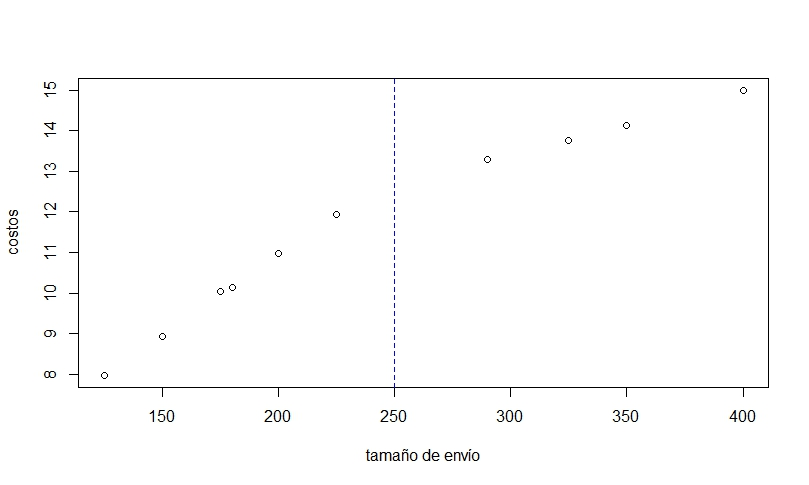
\includegraphics[width=1\linewidth]{imagenes/2_a}
Sí parece razonable que haya dos funciones de regresión diferentes (pero conectadas): una cuando el tamaño de envío es menor que 250 piezas $(x_1<250)$ y otra cuando el tamaño de envío es mayor que 250 mil piezas $(x_1>250)$. Las pendientes son diferentes en ambas regiones; en el caso donde la pendiente es mayor, es decir, la región menor a 250 mil piezas, es evidente que los costos según el tamaño de de envio tiene un aumneto constante, mientras que es menos pronunciada cuando el tamaño de envío es mayor que 250 mil piezas, indicando que el costo de envío por unidad (en miles de partes) empieza a disminuir.


%----b
\item Usando una variable ficticia o dummy y un término de interacción para ayudar a definir el modelo de
regresión lineal por partes. Específicamente, el modelo que ajustaremos es:
$$y_{i}=\beta_{0}+\beta_{1}x_{i1}+\beta_{2}(x_{i1}-250)x_{i2}+\epsilon_{i}$$
donde $x_{i1}$ es el tamaño del envio y $x_{i2}=0$ si $x_{i1}<250$ y $x_{i2}=1$ si $x_{i1}>250$\\

Si suponemos que los datos siguen este modelo, ¿cuál es la función de respuesta media para envíos cuyo
tamaño es menor que 250? ¿Y cuál es la función de respuesta media para envíos cuyo tamaño es mayor que
250? ¿Las dos funciones de respuesta media tienen pendientes diferentes y se conectan cuando $x_{i1} = 250$?.

$$\mu_Y=\beta_{0}+\beta_{1}x_{1}+\beta_{2}(x_{1}-250)x_{2}$$

  

  
Función de respuesta media para envíos cuyo tamaño es menor que 250: $$ \mu_Y \mid (x_1<250)= \beta_0 + \beta_1x_1 + \beta_2(x_1 - 250)(0)=\beta_0 + \beta_1x_1$$
  
Función de respuesta media para envíos cuyo tamaño es mayor que 250: $$ \mu_Y \mid (x_1>250)= \beta_0 + \beta_1x_1 + \beta_2(x_1 - 250)(1)=(\beta_0-250\beta_2) + (\beta_1+\beta_2)x_1$$
  
Como puede observarse, las dos funciones de respuesta media tienen pendientes diferentes:\\
  
La pendiente de la función de respuesta media para envíos cuyo tamaño es menor que 250 es: $\beta_1$.\\

La pendiente de la función de respuesta media para envíos cuyo tamaño es mayor que 250 es: $\beta_1+\beta_2$.\\

Como puede observarse, las dos funciones de respuesta media se conectan cuando $x_{1} = 250$:\\
  
De la primera función se tiene: $\mu_Y \mid (x_1=250)=\beta_0 + \beta_1x_1=\beta_0 + 250\beta_1$.\\

De la segunda función se tiene: $\mu_Y \mid (x_1=250)=(\beta_0-250\beta_2) + (\beta_1+\beta_2)x_1=(\beta_0-250\beta_2) + (\beta_1+\beta_2)250=\beta_0 +250 \beta_1$.\\



%-----c
\item  Obtenga la matriz diseño y encuentre el estimador de MCO. 

\begin{verbatim}
datos$x2=ifelse(datos$x1<250,0,1)
datos$x2s=(datos$x1-250)*datos$x2
datos

library(matlib)
#Matriz diseño:
library(mvtnorm)
library(sasLM)
X1=ModelMatrix(y~x1+x2s,datos)
X<-X1$X
\end{verbatim}

\begin{align*}
X=\begin{bmatrix}
1&225&0\\
1&350&100\\
1&150&0\\
1&200&0\\
1&175&0\\
1&180&0\\
1&325&75\\
1&290&40\\
1&400&150\\
1&125&0\\
\end{bmatrix}
\end{align*}
\begin{verbatim}
#Ajuste del modelo:
m1=lm(y~x1+x2s,datos)
summary(m1)
Call:
lm(formula = y ~ x1 + x2s, data = datos)

Residuals:
     Min       1Q   Median       3Q      Max 
-0.10540 -0.06390 -0.02906  0.08047  0.11811 

Coefficients:
              Estimate Std. Error t value Pr(>|t|)    
(Intercept)  3.2139257  0.1785735   18.00 4.04e-07 ***
x1           0.0384599  0.0009554   40.25 1.52e-09 ***
x2s         -0.0247734  0.0016460  -15.05 1.37e-06 ***
---
Signif. codes:  0 ‘***’ 0.001 ‘**’ 0.01 ‘*’ 0.05 ‘.’ 0.1 ‘ ’ 1

Residual standard error: 0.09303 on 7 degrees of freedom
Multiple R-squared:  0.9988,	Adjusted R-squared:  0.9985 
F-statistic:  2938 on 2 and 7 DF,  p-value: 5.813e-11
\end{verbatim}
%------d
\item Según su función de regresión estimada, ¿cuál es el costo previsto para un envío con un tamaño de 125? ¿un tamaño de 250? ¿con un tamaño de 400?.\\
Convénzase de que obtendrá la misma predicción para tamaño = 250 independientemente de la función de
regresión estimada que utilice.\\

\begin{verbatim}
x1=c(125,250,400)
x2s=ifelse(x1-250>0,x1-250,0)
X=cbind(1,x1,x2s)
yhat=X%*%m1$coefficients
cbind(x1,yhat)
      x1          
[1,] 125  8.021416
[2,] 250 12.828907
[3,] 400 14.881892
\end{verbatim}

Función de respuesta media para envíos cuyo tamaño es menor que 250: $$ \mu_Y \mid (x_1<250)= \beta_0 + \beta_1x_1 + \beta_2(x_1 - 250)(0)=\beta_0 + \beta_1x_1=3.21393+0.03846*x_1$$
  
Función de respuesta media para envíos cuyo tamaño es mayor que 250: $$ \mu_Y \mid (x_1>250)= \beta_0 + \beta_1x_1 + \beta_2(x_1 - 250)(1)=(\beta_0-250\beta_2) + (\beta_1+\beta_2)x_1=9.40643+0.01369x_1$$
  
$\hat{y} \mid (x_1=125)=3.21393 +0.03846*125=8.0214$.\\

Usando la primera función se tiene: $\hat{y} \mid  (x_1=250)=3.21393 +0.03846*250=12.8289$.\\

Usando la segunda función se tiene: $\hat{y} \mid (x_1=250)=9.40643+0.01369*250=12.8289$.

$\hat{y} \mid (x_1=400)=9.40643+0.01369*400=14.8824$.


%-------
\item Grafique sus ecuaciones estimadas sobre la gráfica de dispersión de datos y anote sus predicciones en d).
\begin{verbatim}
plot(y~x1,datos,xlab = "tamaño de envío", ylab="costos")
x1=c(min(datos$x1),250,max(datos$x1))
x2s=ifelse(x1-250>0,x1-250,0)
X<-cbind(1,x1,x2s)
lines(x1,as.vector(X%*%m1$coefficients),col="red",lwd=2)
abline(v=250,col="blue",lwd=1,lty=2)
points(x=125, y=8.0214,type="p", pch=20, col="green")
points(x=250, y=12.8289,type="p", pch=20, col="green")
points(x=400, y=14.8824,type="p", pch=20, col="green")
\end{verbatim}
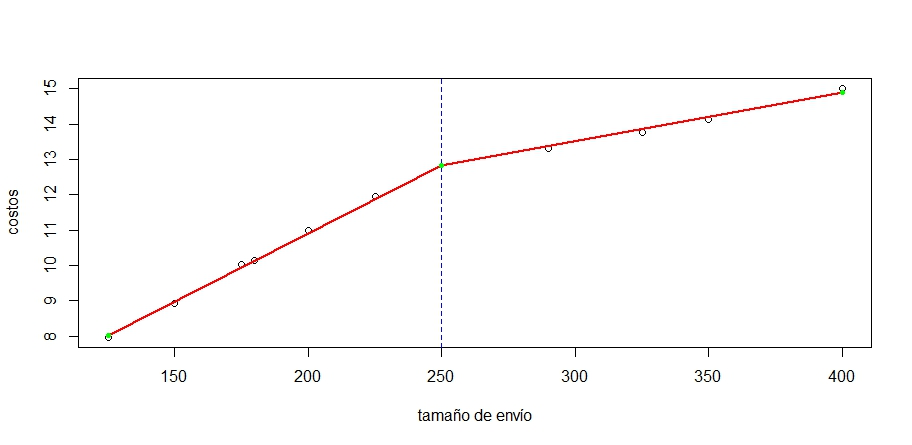
\includegraphics[width=1\linewidth]{imagenes/2_1}
\item ¿Cree que el modelo de regresión lineal por partes resume razonablemente estos datos?. Obtenga un intervalo del 95\% de credibilidad para $\beta_2$ para soportar su respuesta (asuma un enfoque bayesiano).

\begin{verbatim}
m2 <- brm(y~x1+x2s, data = datos)
print(m2, digits = 6)
Family: gaussian 
  Links: mu = identity; sigma = identity 
Formula: y ~ x1 + x2s 
   Data: datos (Number of observations: 10) 
  Draws: 4 chains, each with iter = 2000; warmup = 1000; thin = 1;
         total post-warmup draws = 4000

Regression Coefficients:
           Estimate Est.Error  l-95% CI  u-95% CI     Rhat Bulk_ESS
Intercept  3.213552  0.229582  2.747450  3.678697 1.000698     2412
x1         0.038457  0.001233  0.035924  0.040931 1.001060     2331
x2s       -0.024764  0.002125 -0.029027 -0.020570 1.001215     2313
          Tail_ESS
Intercept     2123
x1            1980
x2s           1746

Further Distributional Parameters:
      Estimate Est.Error l-95% CI u-95% CI     Rhat Bulk_ESS Tail_ESS
sigma 0.115010  0.038355 0.064471 0.207307 1.002189      983     1307
\end{verbatim}

\begin{verbatim}
print(describe_posterior(m2, centrality = "mean")[1:8], digits = 6)
Summary of Posterior Distribution

Parameter   |      Mean |         95% CI |   pd |  ROPE_CI |  ROPE_low
----------------------------------------------------------------------
b_Intercept |  3.213552 | [ 2.75,  3.68] | 100% | 0.950000 | -0.237835
b_x1        |  0.038457 | [ 0.04,  0.04] | 100% | 0.950000 | -0.237835
b_x2s       | -0.024764 | [-0.03, -0.02] | 100% | 0.950000 | -0.237835
\end{verbatim}
\begin{verbatim}
plot(m2)
\end{verbatim}
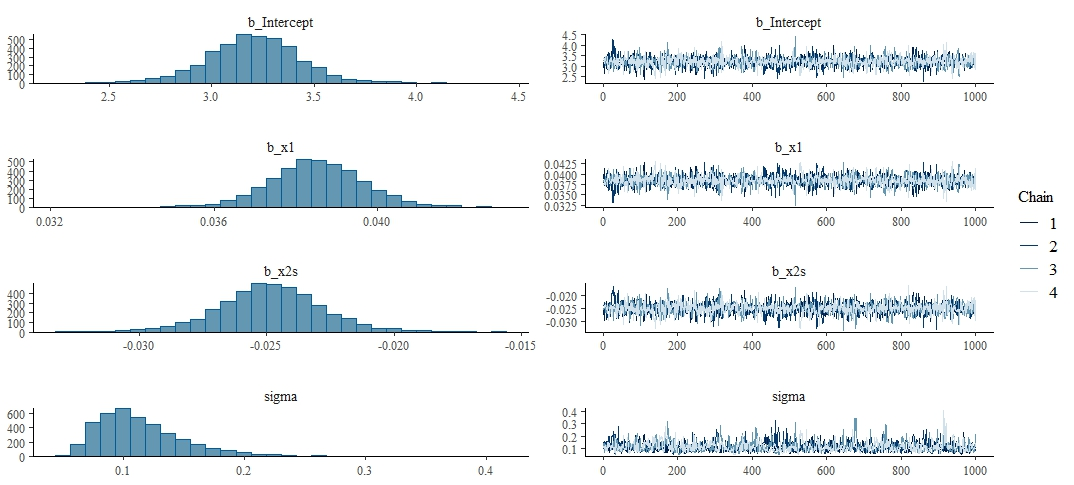
\includegraphics[width=1\linewidth]{imagenes/2_b}
Se obtiene el intervalo de credibilidad.
\begin{verbatim}
#Distribución posterior
posterior_samp <- posterior_samples(m2)
# Calcular beta_2:
posterior_samp$indice <- posterior_samp$b_x2s

#Intervalo de credibilidad del 95%:
cred_interval <- quantile(posterior_samp$indice, c(0.025, 0.975))
# Resultados
knitr::kable(c(mean = mean(posterior_samp$indice), cred_interval))
|      |          x|
|:-----|----------:|
|mean  | -0.0247643|
|2.5%  | -0.0290271|
|97.5% | -0.0205701|
\end{verbatim}
Los resultados obtenidos con el analisis bayesiano son iguales a los de la regresión clásica segmentada. Lo que da soporte al modelo, éste estima los parámetros considerando los dos comportamientos en las regiones de los datos (cuando el tamaño de envio es menor y cuando es mayor de 250 mil piezas). 
\end{enumerate}

%--------EJERCICIO 1------------
\paragraph{Problema 3}
Científicos en Costa Rica están interesados en el proceso de regeneración de bosques en antiguas plantaciones. Una plantación antigua se puede replantar con árboles de rápido crecimiento y luego dejarla sin administrar durante muchos años. Los árboles plantados crecen para y pueden ser cosechados. Con el paso del tiempo,nuevas plantas leñosas crecen debajo de semillas dispersas a los sitios por medios naturales, como animales,vientos y agua. Cuando se cosechan los árboles plantados, las plantas leñosas que crecen debajo pueden regenerar el bosque natural.\\

Los científicos estaban interesados en determinar cuál de las seis especies de árboles comúnmente plantadas promovía la mayor regeneración de bosques medida por la densidad de nuevas plantas leñosas en el sotobosque.\\
Los datos fueron recolectados en tres sitios, La Selva, Paniagua y Quesada. La primera fue una antigua
plantación de investigación y la las dos últimas eran plantaciones de propiedad privada. En cada sitio, se establecieron 30 parcelas y se plantaron cinco parcelas para cada especie de arbol. Las seis especies fueron Calophyllum brasiliense (Cb), Hieronyma alchorneoides (Ha), Terminalia amazonia (Ta), Virola koschnyi (Vk), Vochysia ferruginea (Vf) y Vochysia guatemalensis (Vg). Nueve años después, las parcelas se midieron contando el número total de plantas leñosas en el sotobosque una región de 4 x 4 metros cuadrados dentro de cada parcela. Las parcelas también diferían por otras características. Los árboles fueron plantados en matrices regulares, pero de diferentes dimensiones. Por ejemplo, los árboles plantados en una matriz de 2 x 4 tenían un espacio de 8 metros cuadrados por árbol, mientras que los árboles plantados en una matriz de 4 x 8 tenían un espacio de 32 metros cuadrados por árbol. La mayoría de las parcelas estaban en terreno plano, pero algunos con pendientes de hasta el 10 por ciento. El drenaje en la mayoría de las parcelas es bueno, pero es deficiente en algunas parcelas. Los la cantidad de luz disponible para el sotobosque se midió en cada parcela como un porcentaje de dosel abierto. Los datos para este problema se anexa. Las variables son: 1.tallos, el recuento de tallos leñosos en una parcela de 16 metros cuadrados; 2. sitio, el nombre del sitio; 3. Tratamiento, la especie de árbol plantada (abreviada); 4. espacio, el número de metros cuadrados por árbol plantado; 5. Pendiente, un factor con niveles planos e inclinados; 6. Drenaje, factor con buenos y malos
niveles; y 7. dosel, el porcentaje de dosel abierto.\\\\

La pregunta principal de interés es \textbf{comparar las medidas de regeneración de las seis especies diferentes de
árboles plantados}.\\
\begin{itemize}
%-----------a
\item[a)]Formule un modelo lineal que pueda ayudar a dar una respuesta.\\
\begin{verbatim}
#MODELO CON TODAS LAS VARIABLES (prueba stepAIC 
#para elegir el mejor modelo)
model_completo<-lm(tallos~trat*sitios*espacio*pendiente*drenaje, 
data = datos3)
elecc<-stepAIC(model_completo)

Step:  AIC=338.6
tallos ~ trat + sitios + pendiente + trat:sitios + trat:pendiente

                 Df Sum of Sq     RSS    AIC
<none>                         2492.9 338.60
- trat:pendiente  2     162.1  2655.0 340.21
- trat:sitios     9   13725.9 16218.8 487.27

#De metodo de seleccion se obtiene
tallos ~ trat + sitios + pendiente + trat:sitios + trat:pendiente


> modelo1<- lm(tallos ~ trat + sitios + pendiente + trat:sitios + 
trat:pendiente, data = datos3)
> anova(modelo1)
Analysis of Variance Table

Response: tallos
               Df Sum Sq Mean Sq  F value Pr(>F)    
trat            5   6077  1215.5  33.1549 <2e-16 ***
sitios          2  43472 21735.8 592.8944 <2e-16 ***
pendiente       1     94    94.5   2.5768 0.1131    
trat:sitios    10  21529  2152.9  58.7246 <2e-16 ***
trat:pendiente  2    162    81.1   2.2111 0.1174    
Residuals      68   2493    36.7              

mf<-lm(formula = tallos ~ trat *sitios, data = datos3)
anova(mf)

Analysis of Variance Table

Response: tallos
            Df Sum Sq Mean Sq F value    Pr(>F)    
trat         5   6077  1215.5  31.474 < 2.2e-16 ***
sitios       2  43472 21735.8 562.827 < 2.2e-16 ***
trat:sitios 10  21536  2153.6  55.766 < 2.2e-16 ***
Residuals   71   2742    38.6                      
---
Signif. codes:  0 ‘***’ 0.001 ‘**’ 0.01 ‘*’ 0.05 ‘.’ 0.1 ‘ ’ 1


>summary(mf)

Call:
lm(formula = tallos ~ trat * sitios, data = datos3)

Residuals:
   Min     1Q Median     3Q    Max 
 -13.4   -3.8    0.0    2.6   15.6 

Coefficients:
                      Estimate Std. Error t value Pr(>|t|)    
(Intercept)             94.000      2.779  33.823  < 2e-16 ***
tratHa                 -49.600      3.930 -12.620  < 2e-16 ***
tratTa                 -54.800      3.930 -13.943  < 2e-16 ***
tratVf                 -48.200      3.930 -12.264  < 2e-16 ***
tratVg                  14.400      3.930   3.664 0.000475 ***
tratVk                 -28.000      3.930  -7.124 6.95e-10 ***
sitiosPaniagua         -91.250      4.169 -21.889  < 2e-16 ***
sitiosQuesada          -65.600      3.930 -16.691  < 2e-16 ***
tratHa:sitiosPaniagua   68.250      5.729  11.912  < 2e-16 ***
tratTa:sitiosPaniagua   74.250      5.729  12.959  < 2e-16 ***
tratVf:sitiosPaniagua   46.650      5.729   8.142 9.11e-12 ***
tratVg:sitiosPaniagua    2.650      5.729   0.463 0.645119    
tratVk:sitiosPaniagua   42.650      5.729   7.444 1.79e-10 ***
tratHa:sitiosQuesada    29.200      5.558   5.253 1.49e-06 ***
tratTa:sitiosQuesada    58.400      5.558  10.507 4.15e-16 ***
tratVf:sitiosQuesada    66.200      5.558  11.910  < 2e-16 ***
tratVg:sitiosQuesada   -25.000      5.558  -4.498 2.62e-05 ***
tratVk:sitiosQuesada    24.200      5.558   4.354 4.41e-05 ***
---
Signif. codes:  0 ‘***’ 0.001 ‘**’ 0.01 ‘*’ 0.05 ‘.’ 0.1 ‘ ’ 1

Residual standard error: 6.214 on 71 degrees of freedom
Multiple R-squared:  0.9629,	Adjusted R-squared:  0.954 
F-statistic: 108.3 on 17 and 71 DF,  p-value: < 2.2e-16
\end{verbatim} 
\[Y_{ijkl}= \mu + \tau_i + \alpha_j + (\tau\alpha)_{ij}) + \epsilon_{ijkl}\]
Dónde: 
\item[*] $y_{ij}$ es el tamallo del tallo
\item[*]$\mu$ representa la media general de las respuestas
\item[*]$\tau_i$ representa el efecto de la i-esima especie con $i=1,2,...,6$
\item[*]$\alpha_j$ representa el efecto del j-esimo sitio con $j=1, 2, 3$
\item[*]$(\tau\alpha)_{ij}$ representa la interacción de la i-ésima especie con el j-ésimo sitio 
\item[*]$\epsilon_{ijk}$ error aleatorio asociado con la observación en el sitio \(i\), tratamiento \(j\) y la \(k\)-ésima repetición (parcela), se supone $\thicksim n (0, I\sigma^2)$\\

De lo anterior el modelo desarrollado es: \\
\begin{align*}
 y_{ij} = \mu + \tau_1 + \tau_2 + \tau_3 + \tau_4 + \tau_5 + \tau_6 + \alpha_1 + \alpha_2 + \alpha_3 + (\tau \alpha)_{11}(\tau \alpha)_{12} + (\tau \alpha)_{13}
\\ + (\tau \alpha)_{21}+ (\tau \alpha)_{22} + (\tau \alpha)_{23}+...+ (\tau \alpha)_{61}+(\tau \alpha)_{62} + (\tau \alpha)_{63}
\end{align*}


\item[b)]Utilizando software estime parámetros de su modelo y realice la inferencia para apoyar su respuesta.\\
Para obtener la respuesta se desarrollo: 
\begin{verbatim}
> dim(X)
[1] 89 28
Re<- datos3$tallos
Re
dim(Re)
#Vector de betha
Beta1<-Ginv(t(X)%*%X)%*%t(X)%*%Re
Beta1

pruebatukey<- HSD.test(mf, c("sitios", "trat"), group = T)
pruebatukey
$statistics
   MSerror Df     Mean       CV
  38.61901 71 35.91011 17.30549

$parameters
   test      name.t ntr StudentizedRange alpha
  Tukey sitios:trat  18         5.119798  0.05

$means
            tallos        std r       se Min Max Q25   Q50    Q75
LaSelva:Cb   94.00  4.8989795 5 2.779173  87  99  91  96.0  97.00
LaSelva:Ha   44.40  9.7365292 5 2.779173  35  60  39  41.0  47.00
LaSelva:Ta   39.20  7.7910205 5 2.779173  31  48  31  42.0  44.00
LaSelva:Vf   45.80  5.4497706 5 2.779173  39  53  42  47.0  48.00
LaSelva:Vg  108.40 12.5219807 5 2.779173  95 123  96 111.0 117.00
LaSelva:Vk   66.00  7.6485293 5 2.779173  54  74  65  66.0  71.00
Paniagua:Cb   2.75  0.9574271 4 3.107210   2   4   2   2.5   3.25
Paniagua:Ha  21.40  2.7018512 5 2.779173  17  24  21  22.0  23.00
Paniagua:Ta  22.20  3.1144823 5 2.779173  17  25  22  23.0  24.00
Paniagua:Vf   1.20  0.8366600 5 2.779173   0   2   1   1.0   2.00
Paniagua:Vg  19.80  7.0851958 5 2.779173  15  32  16  16.0  20.00
Paniagua:Vk  17.40  4.3931765 5 2.779173  11  23  16  18.0  19.00
Quesada:Cb   28.40  7.5365775 5 2.779173  21  37  23  25.0  36.00
Quesada:Ha    8.00  3.7416574 5 2.779173   2  12   8   8.0  10.00
Quesada:Ta   32.00  5.1478151 5 2.779173  24  38  31  33.0  34.00
Quesada:Vf   46.40  5.4129474 5 2.779173  38  53  46  47.0  48.00
Quesada:Vg   17.80  5.4037024 5 2.779173  12  24  14  16.0  23.00
Quesada:Vk   24.60  4.1593269 5 2.779173  22  32  23  23.0  23.00

$comparison
NULL

$groups
            tallos groups
LaSelva:Vg  108.40      a
LaSelva:Cb   94.00      b
LaSelva:Vk   66.00      c
Quesada:Vf   46.40      d
LaSelva:Vf   45.80     de
LaSelva:Ha   44.40     de
LaSelva:Ta   39.20    def
Quesada:Ta   32.00    efg
Quesada:Cb   28.40    fgh
Quesada:Vk   24.60     gh
Paniagua:Ta  22.20    ghi
Paniagua:Ha  21.40    ghi
Paniagua:Vg  19.80    ghi
Quesada:Vg   17.80   ghij
Paniagua:Vk  17.40    hij
Quesada:Ha    8.00    ijk
Paniagua:Cb   2.75     jk
Paniagua:Vf   1.20      k

attr(,"class")
[1] "group"
> 
\end{verbatim}
\[ \beta = (XX')^{-1} X' Y\]
\begin{align*}
\beta = \begin{bmatrix}
24.60\\
-14.65\\
4.00\\
4.80\\
-16.20\\
2.40\\
0.00\\
41.40\\
-7.20\\
0.00\\
42.65\\
18.45\\
0.00\\
-25.60\\
-20.60\\
0.00\\
-31.60\\
2.60\\
0.00\\
-4.00\\
38.00\\
0.00\\
40.00\\
-9.20\\
0.00\\
0.00\\
0.00\\
0.00\\
\end{bmatrix}
\end{align*}
\item[c)] Es razonable el uso de su modelo?\\
El analisis para la selección del modelo se hizo utilizando la prueba de selección de variables tomando en cuenta el criterio AIC,
el cual elige al modelo con el AIC más alto, se probó el uso de las variables y sus interacciones, se realizo una prueba de selección de variables tomando en cuenta el criterio AIC. \\


En el modelo se puede comparar las medidas de regeneración, lo cual nos ayuda a tomar decisiones sobre el tipo de especie que podrá generar un mejor efecto de regeneración, como se presenta a continuación: \\
\\
En los resultados del ANOVA se concluye que tanto el sitio como la especie plantada tienen un efecto significativo en la regeneración.
Por las diferencias se realizó una prueba de medias utilizando el método de Tukey \\
\begin{center}
\begin{tabular}{|c|c|c|}
\hline 
Combinación & Media de crecmiento de tallos & Grupo \\ 
\hline 
Selva:Vg  & 108.40 & a\\
\hline 
Selva:Cb & 94.0 & b\\
\hline 
Selva:Vk & 66.0 & c\\
\hline 
Quesada:Vf & 46.40 & d\\
\hline 
Selva:Vf & 45.80 & de\\
\hline 
Selva:Ha &  44.40 & de\\
\hline 
Selva:Ta &  39.20 & def\\
\hline 
Quesada:Ta &  32.0 & efg\\
\hline 
Quesada:Cb & 28.40 & fgh\\
\hline 
Quesada:Vk & 24.60 & gh\\
\hline 
Paniagua:Ta & 22.20 & ghi\\
\hline 
Paniagua:Ha & 21.40 & ghi\\
\hline 
Paniagua:Vg & 19.80 & ghi\\
\hline 
Quesada:Vg  & 17.80 & ghij\\
\hline 
Paniagua:Vk & 17.40 & hij\\
\hline 
Quesada:Ha & 8.00 & ijk\\
\hline 
Paniagua:Cb & 2.75 & jk\\
\hline 
Paniagua:Vf & 1.20 &  k\\ 
\hline 
\end{tabular} 
\end{center}

\begin{center}
%\includegraphics[scale=0.5]{gruposcom.png} 
\end{center}
En la tabla ordenada,se observa que el grado de regeneraión del sotobosque medido por el numero de tallos en el sotobosque será mejor en plantaciones dedicadas a  investigación (La Selva)y que la especie que propicia una mejor respuesta de regeneración será \textit{Vochysia guatemalensis (Vg)}






\end{itemize}

\end{enumerate}
\end{document}